I convenzionali modelli non-supervisionati impiegano rappresentazioni basate su \textbf{Bag of Words}, in cui un documento viene trasformato in un elenco di parole distinte riportandone il relativo numero di occorrenze. Tuttavia, questo approccio comporta ad una valorizzazione della numerosità dei termini, a discapito della vera relazione semantica che li contraddistingue. \vspace{7pt} \\
In risposta a tale problematica, le tecniche di \textbf{text-embeddings}, in cui le informazioni non-strutturate sono riprodotte in un formato numerico, hanno riconosciuto una rapida espansione senza precedenti, divenendo un elemento chiave all'interno della letteratura. A tal proposito, BERT e le sue varianti hanno dimostrato eccellenti risultati in ambito di \textbf{rappresentazioni vettoriali} di dati testuali, mantenendo un elevato significato semantico \cite{grootendorst2022bertopic}. \vspace{7pt} \\
Nell'immagine seguente sono raffigurati alcuni termini semanticamente simili tra loro. Le rappresentazioni vettoriali delle parole \textbf{wolf} e \textbf{dog} sono posizionate in prossimità, poiché appartengono alla stessa famiglia di canidi. Ciò avviene anche per il vettore \textbf{cat}, dato che assieme a dog sono entrambi animali domestici. Contrariamente, sul lato opposto sono riportati vocaboli che non possiedono alcuna similarità con i vettori illustrati fino ad ora. 
\begin{figure}[H]
    \centering
    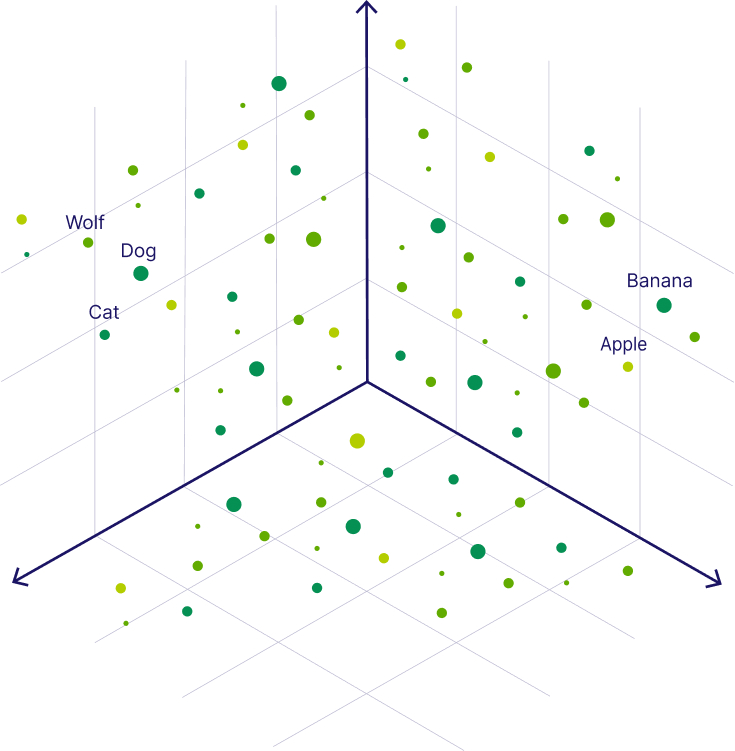
\includegraphics[width=.5\textwidth]{img/img3.png}
    \caption{Raffigurazione vettoriale di informazioni testuali}
\end{figure}
Nonostante i metodi citati possano essere applicati ad una vasta gamma di obiettivi, un possibile scenario d'uso prevede il loro impiego nelle operazioni di \textbf{topic modeling}, finalizzate all'identificazione di temi ricorrenti all'interno di un testo. Un algoritmo in grado di soddisfare una richiesta simile è il modello \textbf{BERTopic}. \vspace{7pt} \\
Il modello genera i topic comuni alla lista di documenti data in ingresso, mediante il conseguimento di tre iterazioni principali.
\begin{itemize}
    \renewcommand{\labelitemi}{-}
    \item \textbf{Conversione dei documenti}. \\
    Il modello inizialmente presuppone che le risorse fornite contengano intrinsecamente temi correlati, in maniera tale che possa dedurre codifiche vettoriali che siano semanticamente confrontabili. La conversione avviene mediante il framework \textbf{SBERT}, il quale permette di trasformare frasi e paragrafi nella propria controparte numerica, utilizzando language models pre-addestrati. I risultati ottenuti sono poi adoperati per raggruppare documenti aventi un significato simile.
    \item \textbf{Raggruppamento dei documenti}. \\
    L'aumento della dimensionalità dei dati causa una minore precisione del quadro delineato nello spazio vettoriale, in cui le distanze differiscono marginalmente tra documenti eterogenei. In queste circostanze è necessario ridurre la dimensione degli embeddings affinché algoritmi di clustering possano operare al meglio delle proprie possibilità.
    \item \textbf{Rappresentazione dei topic}. \\
    Dopo al raggruppamento, ogni cluster è contraddistinto da una serie di possibili topic, rendendo necessario selezionare quelli più pertinenti. Ciò avviene tramite una particolare implementazione della tecnica \textbf{TF-IDF}, utilizzata per valutare la rilevanza di un termine all'interno di un documento, secondo la formula:
    \begin{center}
        $W_t,_d = tf_t,_d \cdot log(\frac{N}{df_t})$
    \end{center}
    dove:
    \begin{itemize}
        \renewcommand{\labelitemi}{-}
        \item \textbf{Term Frequency} ($tf_t,_d$). \\
        Numero di occorrenze di un termine nel documento.
        \item \textbf{Inverse Document Frequency} ($log(\frac{N}{df_t})$). \\
        Misura l'importanza di un termine rispetto all'intera collezione di documenti.
    \end{itemize}
    L'algoritmo BERTopic adotta una procedura simile, ma attuandola a livello di cluster: l'incisività di una parola non è stabilita in base alla completa raccolta di documenti, ma è calcolata impiegando esclusivamente i contenuti presenti all'interno del cluster. Di conseguenza, la formula viene adattata come segue:
    \begin{center}
        $W_t,_d = tf_t,_d \cdot log(1+\frac{A}{df_t})$
    \end{center}
    dove:
    \begin{itemize}
        \renewcommand{\labelitemi}{-}
        \item \textbf{Term Frequency} ($tf_t,_d$). \\
        Immutato rispetto all'equazione precedente.        
        \item \textbf{Inverse Class Frequency} ($log(1+\frac{A}{df_t})$). \\ 
        Determina il peso di un termine rispetto ad una classe di documenti, corrispondente al cluster considerato.
    \end{itemize}
    In sintesi, questa tecnica, nota come \textbf{class-based TF-IDF}, consente di valutare l'importanza delle parole in base a classi di documenti di appartenenza, che in questo contesto sono rappresentate dai cluster individuati in precedenza.
\end{itemize}